\documentclass[margin=5mm]{standalone}
\usepackage[dvipsnames]{xcolor}
\usepackage{pgfplots}
\usepackage{tikz}
\usepackage[tikz]{ocgx2}

\pgfplotsset{compat=1.18}
\begin{document}

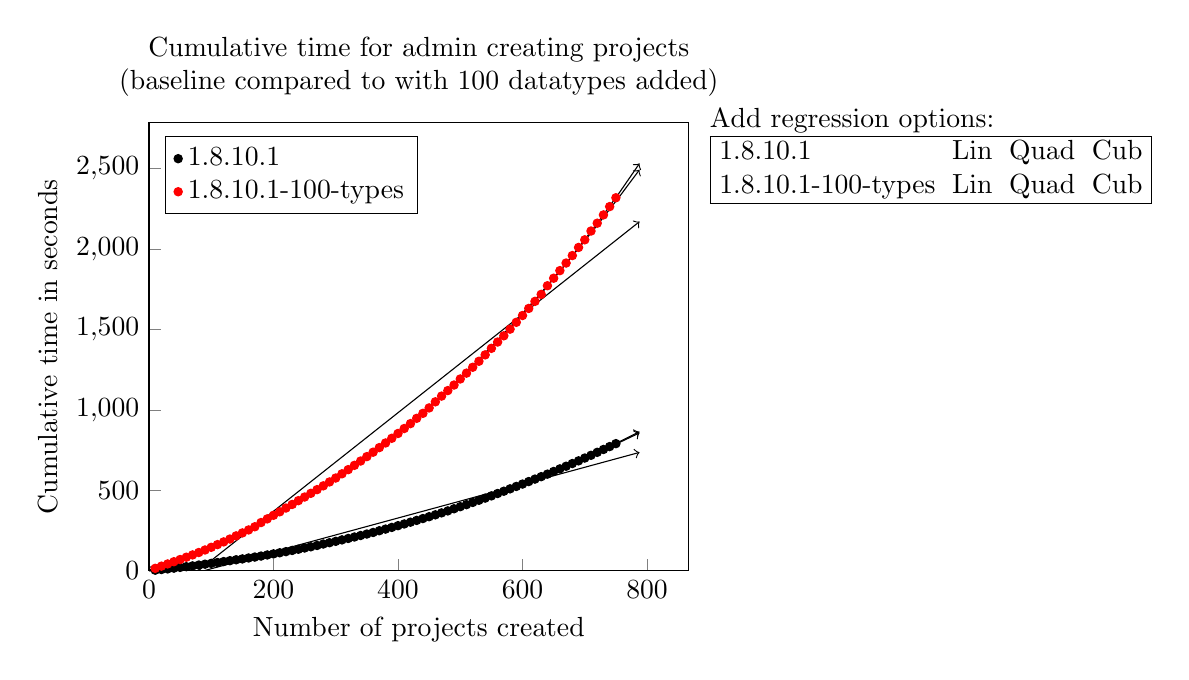
\begin{tikzpicture}
    \begin{axis}[
        align = center,
        legend pos = north west,
        legend cell align = left,
        xlabel = Number of projects created,
        ylabel = Cumulative time in seconds,
        xtick pos = left,
        ytick pos = left,
        scaled ticks = false,
        xmin = 0,
        ymin = 0,
        title = {Cumulative time for admin creating projects (baseline compared to with 100 datatypes added)},
        title style = {text width = 0.8\textwidth},
        legend entries={\switchocg{1.8.10.1}{1.8.10.1},\switchocg{1.8.10.1-100-types}{1.8.10.1-100-types}}]
        \begin{scope}[ocg = {ref = 1.8.10.1-Lin, status = invisible}]
            \plot[domain=0:788,->,forget plot] (\x,{-91.3443113513513509360564057715237140655517578125 + 1.04987387197724046927760355174541473388671875*(\x)^1});
        \end{scope}
        \begin{scope}[ocg = {ref = 1.8.10.1-Quad, status = invisible}]
            \plot[domain=0:788,->,forget plot] (\x,{7.463339888929798604522147797979414463043212890625 + 0.27994412205297114493163235238171182572841644287109375*(\x)^1 + 0.00101306546042667059044639632503503889893181622028350830078125*(\x)^2});
        \end{scope}
        \begin{scope}[ocg = {ref = 1.8.10.1-Cub, status = invisible}]
            \plot[domain=0:788,->,forget plot] (\x,{2.554472081944705319500599216553382575511932373046875 + 0.35497907057571265188045117611181922256946563720703125*(\x)^1 + 0.00076786726826957190684963538984675324172712862491607666015625*(\x)^2 + 0.000000215086133471139396100441109650758253479807535768486559391021728515625*(\x)^3});
        \end{scope}
        \begin{scope}[ocg = {ref = 1.8.10.1, status = visible}]
            \addplot[
                only marks,
                color = black,
                mark = *,
                mark size = 1.5 pt
            ]coordinates {(10,4.696)(20,8.79)(30,12.723)(40,17.292)(50,21.945)(60,26.447)(70,31.42)(80,36.529)(90,41.833)(100,46.976)(110,52.384)(120,58.153)(130,63.668)(140,69.339)(150,74.699)(160,80.459)(170,86.194)(180,92.47)(190,99.239)(200,106.086)(210,112.883)(220,119.879)(230,127.206)(240,134.668)(250,142.385)(260,150.03)(270,158.156)(280,167.228)(290,175.28)(300,183.844)(310,192.794)(320,201.694)(330,210.744)(340,220.019)(350,229.221)(360,238.778)(370,249.548)(380,259.802)(390,270.249)(400,280.961)(410,291.64)(420,302.695)(430,313.794)(440,325.377)(450,336.798)(460,348.383)(470,360.465)(480,372.771)(490,386.08)(500,398.86)(510,411.609)(520,425.251)(530,438.75)(540,452.042)(550,466.026)(560,480.643)(570,494.892)(580,509.688)(590,524.581)(600,539.379)(610,554.857)(620,570.195)(630,585.332)(640,600.99)(650,617.479)(660,633.648)(670,649.944)(680,666.733)(690,683.485)(700,700.846)(710,717.891)(720,736.34)(730,754.077)(740,772.003)(750,790.327)};
        \end{scope}
        \begin{scope}[ocg = {ref = 1.8.10.1-100-types-Lin, status = invisible}]
            \plot[domain=0:788,->,forget plot] (\x,{-240.995807207206865996340638957917690277099609375 + 3.05810794879089531406179958139546215534210205078125*(\x)^1});
        \end{scope}
        \begin{scope}[ocg = {ref = 1.8.10.1-100-types-Quad, status = invisible}]
            \plot[domain=0:788,->,forget plot] (\x,{21.721895075897865723391078063286840915679931640625 + 1.010957021909558051220301422290503978729248046875*(\x)^1 + 0.002693619640633339307189686451238230802118778228759765625*(\x)^2});
        \end{scope}
        \begin{scope}[ocg = {ref = 1.8.10.1-100-types-Cub, status = invisible}]
            \plot[domain=0:788,->,forget plot] (\x,{-4.99906924924930340381479254574514925479888916015625 + 1.4194027697788291764169343878165818750858306884765625*(\x)^1 + 0.00135890613787874162989022241987413508468307554721832275390625*(\x)^2 + 0.00000117080131820578770519771134861475303523548063822090625762939453125*(\x)^3});
        \end{scope}
        \begin{scope}[ocg = {ref = 1.8.10.1-100-types, status = visible}]
            \addplot[
                only marks,
                color = red,
                mark = *,
                mark size = 1.5 pt
            ]coordinates {(10,16.167)(20,29.802)(30,43.412)(40,57.295)(50,70.92)(60,85.206)(70,99.479)(80,114.424)(90,130.046)(100,146.69)(110,163.441)(120,180.343)(130,198.073)(140,217.728)(150,235.965)(160,254.464)(170,274.266)(180,300.582)(190,323.233)(200,345.408)(210,367.124)(220,390.561)(230,412.886)(240,436.367)(250,458.896)(260,481.977)(270,504.915)(280,528.274)(290,552.491)(300,576.957)(310,603.104)(320,628.856)(330,655.61)(340,682.414)(350,709.874)(360,737.162)(370,765.713)(380,794.418)(390,823.572)(400,853.383)(410,884.222)(420,914.548)(430,947.424)(440,978.392)(450,1012.043)(460,1049.951)(470,1085.49)(480,1119.777)(490,1154.196)(500,1191.735)(510,1227.995)(520,1264.5)(530,1301.74)(540,1341.413)(550,1382.081)(560,1421.067)(570,1459.717)(580,1501.076)(590,1543.558)(600,1585.721)(610,1629.59)(620,1673.434)(630,1717.006)(640,1770.61)(650,1817.203)(660,1864.314)(670,1911.481)(680,1957.824)(690,2008.197)(700,2055.686)(710,2110.246)(720,2158.834)(730,2210.296)(740,2261.84)(750,2316.686)};
        \end{scope}
    \end{axis}
    \begin{scope}
        \addtolength{\tabcolsep}{-0.3em}
        \node [below right, shape=rectangle, align=left](regressiontable) at (7,6) {
            Add regression options: \\
            \begin{tabular}{|llll|}
                \hline
                1.8.10.1 & \switchocg{1.8.10.1-Lin}{Lin} & \switchocg{1.8.10.1-Quad}{Quad} & \switchocg{1.8.10.1-Cub}{Cub} \\
                1.8.10.1-100-types & \switchocg{1.8.10.1-100-types-Lin}{Lin} & \switchocg{1.8.10.1-100-types-Quad}{Quad} & \switchocg{1.8.10.1-100-types-Cub}{Cub} \\
                \hline
            \end{tabular}
        };
    \end{scope}
\end{tikzpicture}

\end{document}